\documentclass[a4paper,10pt]{article}
\usepackage[utf8]{inputenc}
\usepackage[toc]{appendix}
\usepackage{graphicx}
\usepackage{a4wide,amsmath,amssymb}
\usepackage{color,hyperref}
\usepackage{placeins}

\newcommand{\todo}[1]{\textcolor{red}{#1}}

%opening
\title{Implementations of fixed parameter tractable algorithms for feedback vertex set}
\author{
	Stefan Majoor (08059008)
	\and
	Huib Donkers (0769015)
	\and
	Henk Alkema (0770862)
	\and
	Xi Junquan
	\and
	Leo van Gansewinkel
	\and
	Christopher Ankomah (0863973)
}
\date{\today}

\begin{document}
\maketitle
\setcounter{tocdepth}{2}
\tableofcontents
\clearpage

\begin{abstract}
This report gives an overview of our solution for track B of the first Parameterized Algorithms and Computational Experiments Challenge. For this challenge, the feedback vertex set problem has been solved. In total, three different algorithms have been implemented, namely: (i) the standard randomized algorithm; (ii) the iterative compression algorithm, and (iii) a solution based on tree decomposition. The solution based upon the tree decomposition was too slow and did not yield any meaningful results. The randomized algorithm worked well for instances with a relatively low $k$.  For larger $k$, iterative compression provided the best solution. Still the algorithm is only able to solve a small subset of the available problem instances. 
\end{abstract}

\section{Introduction} \label{sec:intro}
For track B of the first Parameterized Algorithms and Computational Experiments Challenge~\cite{pace}, we implement three
differentFixed Parameter Tractable (FPT) algorithms to find a smallest Feedback Vertex Set (FVS). The algorithms are a
randomizedalgorithm (section~\ref{sec:rand}), an algorithm using iterative compression (section~\ref{sec:itcomp}), and an 
algorithmusing a dynamic programming approach and a tree decomposition (section~\ref{sec:treewidth}). The first two
algorithms use the size of the optimal solution as the parameter, and the latter uses the treewidth as parameter. We
combine thesealgorithm with a number of preprocessing and kernelization methods described in section~\ref{sec:kern} and
\ref{sec:splitsolve}.

To test our algorithm, a random subset of 100 out of the 230 graphs are published on the PACE Challenge
website~\cite{pace}. These 230 graphs are from various real-world sources, ranging from 30 to 20,000 vertices and from 60 to 90,000 edges, with a median of 300 vertices and 1000 edges. The goal is to solve as many instances as possible using no more than 30 minutes per instance.

\section{Kernelization} \label{sec:kern}
%Let's not describe what each step does like this to save more space for other topics
\todo{Add intro/explanation about there being 4 different kernelization options.}\\
% als korte inleiding voor de overige subsecties. Met en zonder k-dependency -> benoem ook gelijk hun time complexity
% The result of solving the problem on the kernel should either be the same as on the original input, since we ensure that we adjust the size $k$ of our solution accordingly whenever we remove a vertex that should be part of the solution
Preprocessing via data reduction or, more specifically, kernelization as a strategy of coping with hard problems is universally used in almost every implementation. The FVS problem is NP-hard and as is shown by Karp [ref1], its NP-complete for both directed and undirected graphs even if the graphs are unweighted. Due to this intractability, V. Bafna et al. suggest using a polynomial time algorithm for computing a near optimal FVS [ref2]. They show that their factor-2 approximation algorithm called \textsc{ FEEDBACK} is a simple and efficient approximation algorithm that can be implemented to run in $O(min\{|E| log |V |, |V |2\})$ time. Therefore, in coherence with the kernelization reduction rules, an algorithm has been implemented based \textsc{ FEEDBACK} in an attempt to simplify and speed up the detection of solutions to the FVS problem. This approximation is preceded and followed by various reduction rules in the implementation that allow the onfollowing processes of the application to apply their methods to reduced problem instances. Results have shown that the application of the kernelization significantly improved the processing speed of the entire application and, consequently, increased the number of solutions found within an acceptable amount of time in combination with the other processes. \\\\
Note that the problem instances $(G,k)$ that are used are read as multigraphs, which means that they do not support self-loops as opposed to allowing multiple edges between any two vertices. Therefore, if the modification to $G$ caused by a reduction rule would theoretically induce a self-loop, the appropriate vertex inducing that self-loop along with its incident edges are immediately removed from the graph $G$ following the Self-Loop Rule, while adjusting parameter $k$ accordingly.

\subsection{Simple Kernelization} % uitleg basis kernelization en terugkoppeling naar kernelittle
Several basic reduction rules that each make simple changes to the graph have been implemented. The safeness of these reduction follows from Proposition 2 as described by H. Bodlander [ref3]. The simple kernelization process firstly removes isolated vertices $v$ from graph $G$, as well as leaves and their incident edges from $G$. Doing so does not change parameter $k$. Next, if a vertex $v$ has degree two and neighbors $a$ and $b$, possibly allowing $a=b$, then the simple kernelization modifies $G$ by replacing $v$ and its two incident edges with a single edge between its two neighbors $a$ and $b$. Note that if this were to create a self-loop, then the simple kernelization method also removes the vertex $a=b$ and its incident edges and reduces parameter $k$ accordingly. \\\\
In case a value for $k$ is passed on to the kernelization, the simple kernelization function also makes use of the reduction rule that reduces the number of edges between two vertices of the multigraph $G$ down to a number of two where applicable.	
%\subsubsection*{Rule 0-1: The Degree-Zero and Degree-One Rules}
%Firstly, we process problem instances in our implementation by simultaneously performing both the Degree-Zero Rule and the Degree-One Rule. We do this by removing any unconnected vertices we find within a graph $G$. That is to say, if $v$ is an isolated vertex, meaning there is no edge incident to $v$, then remove $v$ from $G$. Furthermore, we also remove leafs from $G$ by removing every $v$ that has degree one along with its incident edge from graph $G$. Applying both of these reduction rules does not change our parameter $k$.
%\subsubsection*{Rule 2: The Degree-Two Rule}
%If a vertex $v$ in $G$ has 2, with neighbors $a$ and $b$ and while possibly allowing $a = b$, then we modify $G$ by replacing $v$ and its two incident edges with a single edge between $a$ and $b$. Unless this modification induces a self-loop, parameter $k$ remains unchanged after applying it. In case this modification would result in the creation of a self-loop, namely when $a=b$, then we immediatly remove it using Rule 3: The Self-Loop Rule and adjust parameter $k$ accordingly.
%\subsubsection*{Rule 3: The Self-Loop Rule}
%If there is a loop on a vertex $v$, then we take $v$ into the solution set and reduce our problem instance $(G,k)$ to the instance $(G - v, k - 1)$. Note that since we deal with multigraphs, our original problem instances $(G,k)$ do not support self-loops, because a multigraph is a non-simple undirected graph in which such loops are not permitted, but in which multiple edges between any two vertices are allowed. Therefore, in our implementation, we simply remove self-loops before they practically ocuur whenever applying any kernelization reduction rule would technically induce a self-loop.
%\subsubsection*{Rule 4: The Multiedge Reduction Rule}
%If there are more than two edges between $u$ and $v$, then we delete all but two of these edges, which does not change our parameter $k$.

\subsection{The 2-Approximation for the Undirected FVS Problem}%ref: http://epubs.siam.org/doi/abs/10.1137/S0895480196305124, karp is ref of V. Bafna et al
\label{sec:2approx}
% 1. Waarom approximation (staat in intro)
% 2. Is uitvoering binnen running time aangegeven door paper (+correctness -> we geven aan waarom die de paper accuraat volgt)
% 3.uitleg data structuren etc
% 4. (voor resultaten) verschil tussen resultaten met en zonder gebruik van approximation
% [point-2:]
Given a graph $(G, w)$ with $G = (V,E)$ and $w$ being the weighted vertices in $V$, any vertex of weight zero is removed from $G$ and placed in the solution set $F$ at the outset of the \textsc{Feedback} algorithm. \textsc{FEEDBACK} then decomposes $(G, w)$ into subgraphs $(G_i, w_i)$’s (in the first While loop) by iteratively subtracting $w_i$ from $w$, removing vertices of weight reduced to zero, adding them into $F$, and cleaning up $G$ by using the CleanUp procedure, which recursively deletes vertices of degree $\leq$ 1, until $G$ becomes empty.\\\\
The implementation of \textsc{Feedback} achieves the same result. First, applies the cleanUp helper function that removes all vertices with degree $\leq$ 1 to produce a clean graph where all remaining vertices have degree $\geq$ 2. Afterwards, it creates a HashMap from the remaining vertices to a default weight value of 1 that is consistently used to modify and track the weights of all vertices within the graph of interest. While the original graph $G$ still con %wordt 1 juli afgemaakt
\todo{TODO:remainder of approximation. Meaning/use of result}

\subsection{Advanced Kernelization}% uitleg geavanceerde kernelization stappen en terugkoppeling naar kernelot
\todo{Remaining Reduction rules}

\subsection{Kernelization Running Time} %kernelot tijd, kernelittle tijd
\todo{Why the choice between kernelot and kernelittle matters}
% Opsomming looptijd van voorheenbesproken onderdelen
% Let uit waarom de keuze tussen kernelot en kernelittle er toe doet
% Let uit waarom, ondanks de nadelen van het gebruik van de extras die kernelot aanbied, kernelot gewenster kan zijn dan kernelittle en vice versa



\section{SplitSolve} \label{sec:splitsolve}
To make the algorithms faster the splitsolve algorithm is implemented.The splitsolve algorithm makes use of the divide and conquer algorithm. It first takes a graph, and removes all edges not part of a cycle, since they do not affect the outcome for the end result. This is done using a dfs from each vertex to itself. Then it detects connected components of the graph. Since the minimal feedback vertex set is equal to the union of the minimal vertex set of the connected components of a graph, the algorithm then calls one of the other algorithms for each of the new graphs. Especially for the randomized algorithm this makes a huge difference in running time, since the new running time is now bounded by the solution size of the largest possible connected component, and not for the solution size for the whole graph anymore. 

\section{Randomized algorithm} \label{sec:rand}
The randomized algorithm as described in the book has been implemented as is described in the book. The original algorithm did only work for a given k. Therefore, to find the smallest k, the algorithm just iterates over all k until it finds a suitable solution. Since it is a randomized algorithm it must have a provable error probability of at most $10^-12$ to qualify for the challenge. Since the original algorithm had an error probability of at most 1/e, the algorithm does 28 times as much runs as described in the book since $(1/e)^x < 10^-12$ for $x \geq 28$.

\subsection{Randomized density algorithm}
\todo{Paragraph removed, because it was causing errors, Stefan, have a look at this}
%Another randomized algorithm is implemented that is very similar to the normal randomized algorithm. To get an idea about what this algorithm does, and why it is better than the normal randomized algorithm, let L = <v1, v2, … , vi> be a sequence of vertices that are removed in one run of the algorithm, where vi is the vertex randomly removed at the ith call of the recursive function. In total $4^k$ such sequences are generated. Since the amount of vertices is much smaller than the amount of generated sequences, there are a lot of sequences that partly overlap with another sequence. For example take the sequence <1, 2, 4> and the sequence <1, 2, 3>. In the normal algorithm both sequences are generated from the full graph, which means that kernelization is called in total 6 times. If we are smart though, we can calculate both sequences with 4 calls to the kernelization by first computing the sequence <1,2> and then calculating both sequences from this graph.

To do this the recursive method gets another parameter which denotes the amount of sequences that still have to be generated from the input graph. So the first call has the full graph and $28 * 4^k$ runs as input. In the method itself rather than removing one vertex, the amount of runs is divided over all the vertices in the kernelized graph using a distribution that reflects the result from taking a random vertex runs amount of time. Then the function is called recursively with the kernelized graph without the vertex for all of the vertices, and the amount of runs that were assigned to that subsequence. In other words, rather than distributing one run of the algorithm, all the runs are distributed according to the generated density. Hence the algorithm is dubbed the randomized density algorithm.

To amount of runs needs to be distributed over the possible subsequences resulting from deleting a vertex in a way that reflects the distribution made by the normal randomized algorithm. To do this the runs are first distributed over the edges. This is done by iterating over the edges, and assign an amount of r runs where r is binomial distributed with the amount of trials equal to the amount of not yet distributed runs, and the success probability equal to 1 divided by the amount of edges that still need runs distributed. (This is another way to simulate the distribution of throwing a die with one side for each edge). Then the edge itself distributes the runs assigned to it over its edges using the same formula (i.e. simulating throwing a coin for the assigned amount of runs).,

\subsection{Problems}
The algorithms above have two problems. The first problem is that the lower bound of the algorithm is equal to the upper bound of the algorithm, since in order to verify that k is the lowest possible size vertex set, it first needs to verify that there is no vertex set with size k-1. This can only be done by running the problem at least $28*4^(k -1)$ times. A smarter algorithm might see that such a vertex set is not possible a lot faster. Therefore the algorithm does not work as fast as some other algorithms.

The second problem is related to the randomized density algorithm. Mathematically the distribution of the runs is sound in the sense that it does not affect the probability that the algorithm gives an incorrect answer. However, in the real world this is not possible. The algorithm relies on the discrete binomial distribution. However, it is not possible to generate a random variable from this distribution. To solve this a Guassian distribution is used, with a Z transformation and continuity reflection correction to approximate the binomial distribution. However, since it is an approximation this affects the probability that our algorithm gives an incorrect answer in such a way that we can not guarantee the necessary bound anymore. 

\section{Iterative compression} \label{sec:itcomp}
%FVS - feedback vertex set
%optimal FVS - FVS with smallest size possible
%The graph - problem instance

An algorithm with a time complexity of $O(5^kn^{O(1)})$ has been implemented. This algorithm makes use of the iterative compression approach, where $O(n)$ iterations take place, adding one vertex to the graph every iteration until we reach the original graph again. Let $v_i$ denote the $i$th vertex, based on some arbitrary ordering. For iteration $i$, let $G_i$ be the graph induced by the first $i$ vertices of the original graph $G$. In the first iteration we have an empty graph $G_0$ and a trivially correct and optimal FVS $C_0 = \emptyset$. In each subsequent iteration $i>0$ we find a FVS $C_i$ for the intermediate graph $G_i$, by first obtaining the FVS $C_{i-1} \cup \{v_i\}$. When this FVS is larger than some given integer $k$, we apply a compression algorithm on the intermediate FVS $C_{i-1} \cup \{v_i\}$ to find a smaller solution, or conclude that no smaller solution is possible. This algorithm find a FVS of size at most $k$, or concludes that no such solution exists. To find an optimal solution, this $k$ should be equal to the size of the optimal solution. This problem is solved in section~\ref{sec:noK}.

In every iteration $i$, the compression algorithm is tasked to find a FVS for a graph $G_i$ that is smaller in size than a given FVS $X_i = C_{i-1} \cup \{v_i\}$. It achieves this by iterating over every non-empty subset $Z$ of $X_i$. It labels all vertices in $Z$ as `prohibited', meaning we attempt to find a FVS of a small enough size that does not include any vertex from $Z$, but does include every other vertex in $X_i$. Since $Z$ is a FVS for $G_i-(X_i\setminus Z)$, we can apply the {\sc DisjointFVS} algorithm \todo{FROM THE BOOK} to find such a FVS or conclude that no such FVS exists.

\subsection{Finding the optimal solution without knowing its size}
\label{sec:noK}
Since we don't know the size of the optimal solution, we use the compression algorithm every iteration to maintain an optimal solution for the intermediate graphs. This way we can guarantee that the final solution is optimal. We know that the size of an optimal FVS for $G_i$ is at most one larger than the size of an optimal solution for $G_{i-1}$, since only one vertex was added to the graph. In the best case the size of the optimal solution remains the same. Hence given that $C_{i-1}$ is an optimal solution for $G_{i-1}$ we obtain an optimal solution for $G_i$ by compressing $C_{i-1} \cup \{v_i\}$. When the compression succeeds, we have obtained a FVS of size $|C_{i-1} \cup \{v_i\}|-1 = |C_{i-1}|$, because no smaller FVS can exist. When the compression fails we know there is no solution of size $|C_{i-1}|$ and therefore $C_{i-1} \cup \{v_i\}$ is an optimal solution. Hence when $C_{i-1}$ is optimal for $G_{i-1}$, $C_i$ is optimal for $G_i$. Since $C_0$ is trivially optimal for $G_0$, we conclude that $C_i$ is optimal for $G_i$ for all iterations $i$. Also observe that $|C_{i-1}| \leq |C_i| \leq |C_{i-1}|+1$.

\subsection{Improvements}
Although running the compression algorithm every iteration does not change the worst case running time of the algorithm, running the compression algorithm every iteration might considerably increase the actual running time. However, it turns out that maintaining an optimal solution for every intermediate graph also has its benefits. 

\subsubsection{Reuse old solution when possible}
We have observed that $|C_{i-1}| \leq |C_i| \leq |C_{i-1}|+1$. An easy improvement is to check whether $C_{i-1}$ is a FVS of $G_i$. If this is the case, we know that $C_{i-1}$ is an optimal solution for $G_i$ and assign $C_i = C_{i-1}$, skipping the compression algorithm for this iteration.

\subsubsection{Skip half the work}
For another improvement, observe that when in the compression algorithm, a non-empty subset $Z$ of $X_i$ does not include $v_i$, meaning $v_i \in X_i\setminus Z_i$, the {\sc DisjointFVS} algorithm is run on graph $G_i-(X_i\setminus Z)$ with prohibited vertices $Z$. Observe that $G_i-(X_i\setminus Z) = G_{i-1}-(X_{i-1}\setminus Z)$ when $v_i \not\in Z$. If {\sc DisjointFVS} would return that there exists a FVS $C$ for $G_i-(X_i\setminus Z)$ with $|C|<|Z|$, then this $C$ is also a FVS for $G_{i-1}-(X_{i-1}\setminus Z)$, meaning $C \cup (X_{i-1}\setminus Z)$ is a FVS for $G_{i-1}$ of size $|C \cup (X_{i-1}\setminus Z)| < |X_{i-1}|$. Since there cannot be a FVS for $G_{i-1}$ smaller than $X_{i-1}$, this is a contradiction, hence {\sc DisjointFVS} will return that there is no solution when $v_i \not\in Z$. This means we can skip the half of all non-empty subsets of $X_i$ that do not include $v_i$, speeding up the algorithm by almost a factor $2$. To be able to apply this strategy, the compression algorithm needs to be told which vertex has been added since the last compression.

Note that this strategy can also be applied when we are not applying the compression every iteration, but we would have to consider a set of multiple vertices added since the last compression, instead of only a single one. This means only a very small part of the subsets of $X_i$ (those containing all the vertices added since the last compression) can be skipped.

\subsubsection{Check for cycles only at the start of the recursion}
The {\sc DisjointFVS} algorithm is recursive. Before any reduction rules are applied to the graph, the algorithm checks for cycles in the set of prohibited vertices. If there is a cycle, then there cannot be a FVS that does not contain any of the prohibited vertices. This check is only required in the very first layer of the recursion. No cycles will be added when going deeper in the recursion. New vertices can be labelled a `prohibited', but these never introduce cycles. Checking only at the start of the recursion saved some time.

\subsubsection{Ordering the vertices}
Because we can skip the costly compression algorithm when the old solution is still valid in the new graph, the ordering we choose for the vertices makes a large difference. Since the compression algorithm is triggered only when the new vertex introduces a cycle that does not include a vertex in the old solution, we want an order such that the time number of vertices that introduce such a cycle is low. Since the running time of the compression algorithm is exponential in $k$, the number of vertices that introduce such a cycle \emph{after} the intermediate solution grew is more important than before. This can be achieved in two ways:
\begin{itemize}
 \item Postpone increasing the size of the solution. Doing $3$ compressions with $k=10$ for example takes less time than a single compression with $k=11$.
 \item Attempt to find a `future proof' solution. With this we mean a solution that is likely to be a FVS for graphs in later iterations. Best would be an order where at each step the intermediate solution is a subset of the final optimal solution, meaning we have only $k$ compression steps.
\end{itemize}
We have experimented with a number of ways to define an order on the vertices, based on their degree in $G$ and their weight given by \todo{THE APPROXIMATION ALGORITHM}. For degree and weight we tried increasing and decreasing order and tried all 8 lexicographic orderings on degree and weight. Out of these 12 ordering, the lexicographic ordering on increasing degree then increasing weight was fastest.

We also tried to use a 2-approximation solution to skip a large number of vertices. Set set of vertices no in this 2-approximation form a forest by definition, hence we can safely add all these vertices without compression. Now we have at most $2k$ iterations left in which we may need to compress. Ordering these last $2k$ vertices using the same lexicographic ordering on increasing degree then weight resulted in no significant gain in speed. Since this method actually guarantees at most $2k$ compression steps, we chose to leave this in.

\subsection{Future improvements}
\subsubsection{Reorder vertices on the go}
Since in theory there is no need to define the complete ordering on vertices on beforehand, it may be good to only determine which vertex is the $i$th vertex when we have completed the first $i-1$ iterations. Findings in these earlier iterations may suggest a new order is more likely to reduce the number of costly compressions. Because one of our initial design decisions prevented us from efficiently redefining the order, so we where unable to try this method.

\subsubsection{Use different orderings in parallel}
When something uncontrollable has a large influence on the running time, one can perform a number of independent runs in parallel and stop when one of the runs terminates, returning a solution. Since we are only allowed one thread, we would need to interleave these parallel runs, this slows down each run, but the variance in running times of the different runs may compensate this, resulting in a faster expected running time. In our case however, the variance of the different orders on the vertices is not large enough. However, it the case of iterative compression, it may be possible to devise some methods to estimate how long a given run is going to take. This method can also take information from the parallel runs into account. With such a method, it may be possible to distinguish between fast and slow runs before they terminate. This means we can kill slow runs sooner, which in turn might mean the variance of the different ordering might outweigh the additional running time caused by interleaving.

\subsubsection{Subset iteration}
In our current implementation, the order in which we iterator over all possible subsets of the to be compressed solution is fixed in such a way that for every next subset, only one vertex is added or removed. Since performing more operations to obtain the next subset will not have a significant impact on the running time, they may be a large advantage in changing the order in which we iterate over the subsets. Since we have access to information from previous compressions, we may be able to estimate which subsets are more likely to be successful. Depending on how good this estimation is, trying these subsets first can speed up the compression by a lot.

\subsubsection{Implement reduction rule 4}
THE BOOK describes a fourth reduction rule that can be applied within {\sc DisjointFVS}, resulting in an algorithm for FVS that runs in $O(3.6181^kn^{O(1)})$. \todo{IT IS UNCLEAR WHETHER THIS WILL RESULT IN A FAST ALGORITHM FOR THE VALUES OF $k$ THAT WE ENCOUNTER.} Unfortunately, we didn't get to implementing this in the time available.


\section{Tree decomposition algorithm} \label{sec:treewidth}
\subsection{Making a tree decomposition} \label{sec:treewidth1}
In order to run an algorithm on a tree decomposition of a graph, one first needs such a tree decomposition. To do so, we implemented the algorithm in the given paper.

The algorithm works recursively. Let a connected graph $G = (V,E)$ and a list $(v_1, ... , v_n)$ of the vertices in $V$ be given. If $|V| = 1$, return a bag $X_{v_1} = \{v_1\}$. Else, let $G' = (V',E')$ be the graph found by eliminating $v_1$, that is, by connecting all pairs of neighbours that were previously unconnected and then deleting $v_1$ itself. Now, let $T'$ be the tree decomposition found on $(G',(v_2,...,v_n))$ by this algorithm. Construct a new bag with $v_1$ and all of its neighbours in $G$. Let $v_i$ be the lowest numbered of these neighbours. Then, connect the new bag to the bag $X_{v_i}$ in $T'$ to form the tree decomposition $T$ of $G$. Finally, return $T$.

So, why is the returned tree decomposition a correct tree decomposition? Note that the returned tree decomposition has $|V|$ bags $X_{v_1},...X_{v_n}$. Let us check all requirements one by one:
\begin{itemize}
\item \textbf{Each $v \in V$ is in at least one bag.}\\
	This holds, since $\forall i: v_i \in X_{v_i}$.
\item \textbf{For every edge $(v_i, v_j)$ in the graph, there is a bag that contains both $v_i$ and $v_j$}\\
	Let (w.l.o.g.) $v_i$ be the lowest numbered vertex. Note that eliminating a vertex $v$ from a graph will never delete any edge that does not have $v$ as one of its end points, so the edge $(v_i,v_j)$ in the original graph will not be deleted until $v_i$ is eliminated. Therefore, when $v_i$ is the first vertex in the remaining vertex list, both $v_i$ and $v_j$ are added to the bag $X_{v_i}$. 
\item \textbf{$\forall v \in V$, the subgraph formed by only taking bags that include $v$ is a tree}\\
	Let $v_i \in V$. We will do a short proof by induction over the size of $V$.
	\begin{itemize}
		\item \textbf{Base case}\\
		Suppose $V = \{v_i\}$, then the returned tree decomposition is only a single bag, so the statement holds.
		\item \textbf{Induction step, case 1}\\
		Suppose $v_i$ is not in the newly created bag $X_{v_1}$, i.e.: it is not $v_1$, nor is it a neighbour of $v_1$. Since the statement holds for $T'$ (induction hypothesis), and $X_{v_1}$ (which does not contain $v_i$) is added as a leaf, the statement still holds for $T$.
		\item \textbf{Induction step, case 2}\\
		Suppose $v_i$ is in the newly created bag $X_{v_1}$, but not equal to $v_1$ itself. In other words: it is a neighbour of $v_1$. This bag is then connected to $X_{v_j}$, where $v_j$ was the lowest numbered neighbour of $v_1$. Now, since the statement holds for $T'$ (induction hypothesis), the statement holds iff $X_{v_j}$ contains $v_i$. If $i = j$, then this is clearly true. Else, after the elimination of $v_1$, $v_i$ and $v_j$ are connected. Then, as was proven for the previous tree decomposition requirement, $X_{v_j}$ will contain $v_i$. Therefore, in both cases the statement still holds for $T$.
		\item \textbf{Induction step, case 3}\\
		Suppose $v_i$ is $v_1$. Since $v_i$ is scheduled for elimination, the newly created bag will be the only bag containing $v_i$, so the statement holds for $T$.
	\end{itemize}
	
\end{itemize}
Therefore, the returned tree decomposition is in fact a tree decomposition.

As one might expect, the given order $(v_1,...,v_n)$ has a significant impact on the treewidth of the returned tree decomposition. Luckily, the order of the vertices can also be chosen at runtime. In the paper, multiple ways to chose the order were given. As a test, only the easiest one - choose the vertex with the lowest degree - was implemented.

During the implementation, two small improvements were made. First of all, the algorithm expects a connected graph. One can extend this to all graphs: when $|V| > 1$ and no neighbours are found when creating a new bag $X_{v_i}$, simply add an edge $(v_i,v_j)$ for a random $v_j \in V, v_j \neq v_i$. Of course, by introducing random edges, one might decrease the quality of the returned tree decomposition, so further improvements can probably be made.
Secondly, the recursive structure of the algorithm can easily cause a stack overflow on larger graphs - the recursion depth is always equal to $|V|$ -, so the structure was slightly changed to make the algorithm non-recursive.

Since the algorithm using the tree decomposition turned out to use an abysmal amount of storage no matter the quality of the tree decomposition (see \ref{sec:treewidth2}), no further improvements were made. 

\subsection{Finding a FVS using a tree decomposition} \label{sec:treewidth2}

\subsection{Comparing treewidths and FVS sizes} \label{sec:treewidth3}
Given a FVS of graph $G$ of size $k$, it is easy to see that the treewidth of $G$ is at most $k+1$ using the `cops and robbers' definition: after placing $k$ cops at the nodes of the FVS, two more cops are needed to chase the robber through the remaining forest. However, a small treewidth does not guarantee a small FVS: a set of $n$ loops has a treewidth of 2, but a FVS of size $n$.

We compare the treewidths $w$ of the found tree decompositions (note that $w$ is only an upper bound on the treewidth of $G$) with the found FVS sizes $k$:

~\\\begin{tabular}{|l|l|l|}
\hline
\textbf{Problem} & \textbf{k} & \textbf{w}\\
\hline
003 & 10 & 5 \\
006 & 11 & 10 \\
020 & 8 & 3 \\
028 & 8 & 3 \\
031 & 33 & 4 \\
042 & 11 & 4 \\
050 & 7 & 5 \\
072 & 9 & 10 \\
083 & 7 & 5 \\
085 & 51 & 4 \\
091 & 21 & 6 \\
095 & 8 & 3 \\
096 & 6 & 3 \\
099 & 8 & 4 \\
\hline
\end{tabular}\\

For none of the problems, $w > k+1$, so the tree decomposition probably performs adequately. However, with problem 085 being the clearest example, some problems have a $k$ much bigger than $w$.

\section{Dynamic programming} \label{sec:dynamic program}
\subsection{Improving dynamic programming for FVS} \label{sec:dynamic programming}
Firstly, we decided to follow the option 1 suggested by lecturer for implementing dynamic programming for FVS problem.

\noindent This program is aimed to solve the decision variety of FVS problem:

\noindent [Given an undirected graph $G=(V,E)$ and an integer $k$, whether there exists a set $Y\subset V$ of cardinality $k$ so that $G[V / Y]$ is a forest.]

\noindent In order to make the algorithm working, a nice tree decomposition based on undirected graph $G$ is required, Which will be given by Henk's package.

\noindent We will use the cut\& count to solve the problem based isolation lemma.

\noindent Cut(with integer $A,B,C,W$),$M$ is Marked sets which contains at least one vertice from each loop in $G$ we define like below:
\newline 1) First is the family candidates of solutions:$R_{W}^{A,B,C}$ is the family of pairs $(X,M)$, where $X\subset V/S$, $|X|=A$,$G[X]$ contains $B$ edges,$M\subset X$,$|M|=C$,and $w(X x \{F\})+w(M x \{M\})=W$
\newline 2) $S_{W}^{A,B,C}$ is the solutions which belong to $R_{W}^{A,B,C}$ and $G[X]$ is a forest containing at least one marker from the set $M$ in each connected component.
\newline 3) $C_{W}^{A,B,C}$ is the number of consistent cuts of $X$ for each candidate in $R_{W}^{A,B,C}$.

\noindent Then we construct a function to calculate $C_{W}^{A,B,C}$:$A_x(a,b,c,w,s)$.

\noindent We have $0\leq a \leq |V|$,$0\leq b \leq |V|$,$0\leq c \leq |V|$,$0\leq w \leq  2N|V|$ and s is the status for consistent cut of vertices in Bag $X$.

\noindent With the nice tree decomposition as input,the algorithm works recursively to calculate the function for each bag.

\noindent For each bag, it contains $|B_x|$ vertices, which have $3^|B_x|$ possible status for allocating all vertices into cut 1 or cut 2 or out of $X$,(if in cut 1 is $(v,1)$,if in cut 2 is $(v,2)$, else if not in $X$ is $(v,0)$. And $s(v)$ represents the allocation of $v$.For each possible status, we initial a matrix to store all function value of $A_x(a,b,c,w)$.

\noindent Recursive part based on nice tree decomposition of the whole algorithm($y$ is the child node of $x$):

\noindent Since time limited, follow the suggestion of lecturer, this version of program firstly focus on path decomposition which means there is no join node included.
\begin{itemize}
\item[-] Leaf bag:
Only one possible status for allocating vertices into cuts, $s_x$ only have one element $\emptyset$. And the matrix correlate with $\emptyset$ should be: 

\noindent $A_x(0,0,0,0)=1$,and all other available cell is 0. 
\item[-] Introduce vertex bag($v$):
$v$ is the introduced vertex, we need to take all elements of $s_y$, for each element $s_y(i)$, we made 3 copies, for each copy add one possible allocation of $v$ separately($(v,0)$,$(v,1)$,$(v,2)$). Then based on the allocation of $v$, matrix of each new element could me modified as below:

\noindent if $(v,0)$,keep the matrix of $s_y(i)$.$A_x(a,b,c,w)=A_y(a,b,c,w)$

\noindent if $(v,1)$ or $(v,1)$,for all $0\leq a-1 \leq |V|$ and $0\leq w-w((v,F)) \leq  2N|V|$,$A_x(a,b,c,w)=A_y(a-1,b,c,w-w((v,F)))$, the other cells of matrix is 0.

\item[-] Introduce edge bag($uv$):
Check $s_y$:

\noindent If we have $s(u)=s(v)\neq 0$,for all $0\leq b-1 \leq |V|$ ,$A_x(a,b,c,w)=A_y(a,b-1,c,w)$, the other cells of matrix is 0.

\noindent If we have $s(u)=0$ or $s(v)=0$,keep the matrix of $s_y(i)$.$A_x(a,b,c,w)=A_y(a,b,c,w)$

\noindent else we if not ($s(u)=0$ or $s(v)=0$ or $s(u)=s(v)$), cells in the matrix should be all 0.

\item[-] Forget bag($v$):
For each element in $s_x$, we can find 3 elements in $s_y$($s_x\cup (v,0)$,$s_x\cup (v,1)$,$s_x\cup (v,2)$.

\noindent Then for matrix of $s_x\cup (v,1)$, we first do a copy called $M1$ and then transform as below:
For all $0\leq c-1 \leq |V|$ and $0\leq w-w((v,M)) \leq  2N|V|$,$A_x(a,b,c,w)=A_y(a,b,c-1,w-w((v,M)))+A_y(a,b,c,w)$, the other cells will take original value, $A_x(a,b,c,w)=A_y(a,b,c,w)$.

\noindent Then we make copies called $M2$ of matrix of $s_x\cup (v,0)$, $M3$ of matrix of $s_x\cup (v,2)$.

\noindent Finally, matrix of each element of $s_x$ will be $M1+M2+M3$.

\end{itemize}
Then the whole structure of algorithm will be like:
\newline 1) Read undirected graph $G$, constructing path decomposition $P$,Initial two tables for each vertices in $G$, store weights value of forest and marker separately.
\newline 2) Initial a queue $Q$, add root bag of $P$ in $Q$. While $Q$ is not empty, poll a element $x$ and call recursive function based on the type of node.
\newline 3) If the child node $y$ of $x$ has not been calculated, then add $y$ into $Q$, poll a new element of $Q$, call recursive function again.
\newline 4) If the child node $y$ has already been handled, then get result of recursive function,storing it into entry tables, add $x$'s parent node into $Q$,poll a new element of $Q$.
\newline 5) Repeat the above three steps, then root node will be calculated. Check the matrix of root node, if existing cell modulo 2 is 1, then the output of algorithm is yes, otherwise no.

\noindent Running time:
Since all possible status of $s$ is $3^k$,handling matrix $|A|=n$,$|B|=n$,$|C|=n$,$|w|=8*n^2$,number of nodes will be $O(n)$,the total running time would be $3^k*8*n^6$. So far this algorithm is based on path decomposition, then $k=n$, so final running time is $3^n*8*n^6$.Storage: Also $3^n*8*n^6$.

\noindent Conclusion:
The dynamic algorithm has been corrected implemented based on path decomposition, while because there is no join node which make $k$ very big, so the actual running time and storage is not quite good. With 8g memory the algorithm could handle a graph with 7 vertices in 35 seconds, if more than 7 vertices ,error called "out of heap memory" will happen.

\noindent I think my old way to realize this algorithm could be improved by re-design. If I can redo this program, I will not maintain same size matrix for all nodes, for example leaf node will only have one cell for matrix $A_x(0,0,0,0)=1$, it may save many wasted storage with a little sacrifice of searching time. And also the join node should be solved ,so that algorithm could work on nice tree decomposition instead of path decomposition.




\section{Comparison} \label{sec:comparison}
To test the different algorithms 7 different graphs were determined that were relatively easy to solve. The reason that relatively easy graphs were taken was because not all algorithms gave an answer for the larger graphs. The chosen graphs were then solved 10 times by each algorithm, and the average solving time was taken to compare the algorithms. 

~\\\textbf{Running time full algorithm} \\
The following table gives an overview of the time it took each algorithm to solve the problem in their final form.

~\\\begin{tabular}{|l|l|l|l|l|}
\hline
\textbf{Problem} & \textbf{k} & \textbf{Randomized} & \textbf{Randomized Density} & \textbf{Iterative Compression} \\
\hline
096 & 6 & 695 ms & 107 ms & 40 ms \\
099 & 8 & 743 ms & 168 ms & 6 ms \\
050 & 7 & 4.407 ms & 8.515 ms & 37 ms \\
062 & 7 & 3.857 ms & 1.591 ms & 39 ms \\
083 & 7 & 4.897 ms & 12.798 ms & 12 ms \\
095 & 8 & 17.159 ms & 8.851 ms& 40 ms \\
028 & 8 & 18.124 ms & 9.994 ms& 40 ms \\
\hline
\textbf{Total:} & & 49.882 ms & 40.433 ms & 214 ms\\
\hline
\end{tabular}

~\\\\\textbf{Split Algorithm} \\
To show that the split algorithm works the iterative compression is run on all the instances that it could solve within 20 seconds. Then the iterative compression was run without doing splitsolve first. These were the results:

~\\\begin{tabular}{|l|l|l|l|l|}
\hline
\textbf{Problem} & \textbf{k} & \textbf{Without Split Solve} & \textbf{With Split Solve} & \textbf{Change} \\
\hline
003 & 10 & 396 ms & 401 ms  & +1,2\% \\
006 & 11 & 2827 ms & 1.127 ms & -60.13\% \\
020 & 8 & 35 ms & 27 ms &  -35.71\% \\
028 & 8  & 47ms & 42 ms & -10.64 \% \\
031 & 33 & $>$ 5 min & 153 ms & $>$ -99.95\% \\
042 & 11 & 246 ms & 142 ms & -42.28 \% \\
050 & 7 & 12 ms & 14 ms & 16.67\% \\
072 & 9 & 521 ms & 509 ms & -2.3\% \\
083 & 7 & 9 ms & 10 ms & 11.11\% \\
085 & 51 & $>$ 5 min & 34 ms & $>$ -99.98\% \\
091 & 21 & $>$ 5 min & 2.037 ms & $>$ - 99.32\% \\
095 & 8 & 33 ms & 38 ms & 15.15\% \\
096 & 6 & 9 ms & 11 ms & 22.22\% \\
099 & 8 & 17 ms & 6 ms & -64.71\% \\
\hline
\end{tabular}


%\section{Conclusion} \label{sec:conclusion}

\begin{thebibliography}{9}
 \bibitem{ftpbook}
 Marek Cygan, Fedor V. Fomin, Lukasz Kowalik, Daniel Lokshtanov, Dániel Marx, Marcin Pilipczuk, Michal Pilipczuk and Saket Saurabh. \textit{Parameterized Algorithms}. Springer International Publishing Switzerland 2015
 \bibitem{pace}
 The first Parameterized Algorithms and Computational Experiments Challenge. \url{https://pacechallenge.wordpress.com/track-b-feedback-vertex-set/}
\end{thebibliography}

\clearpage
\appendix

\FloatBarrier
\section{Experimental results Iterative Compression} \label{app:itcomp}
I ran iterative compression about 8000 times with different configurations, on different graphs. \todo{A summary of the results will be inserted here}

\FloatBarrier
\section{Experimental results Dynamic programming} \label{app:dynamicprogram}
Results for 5 vertices graph:
\begin{figure}[H] 
  \centering
  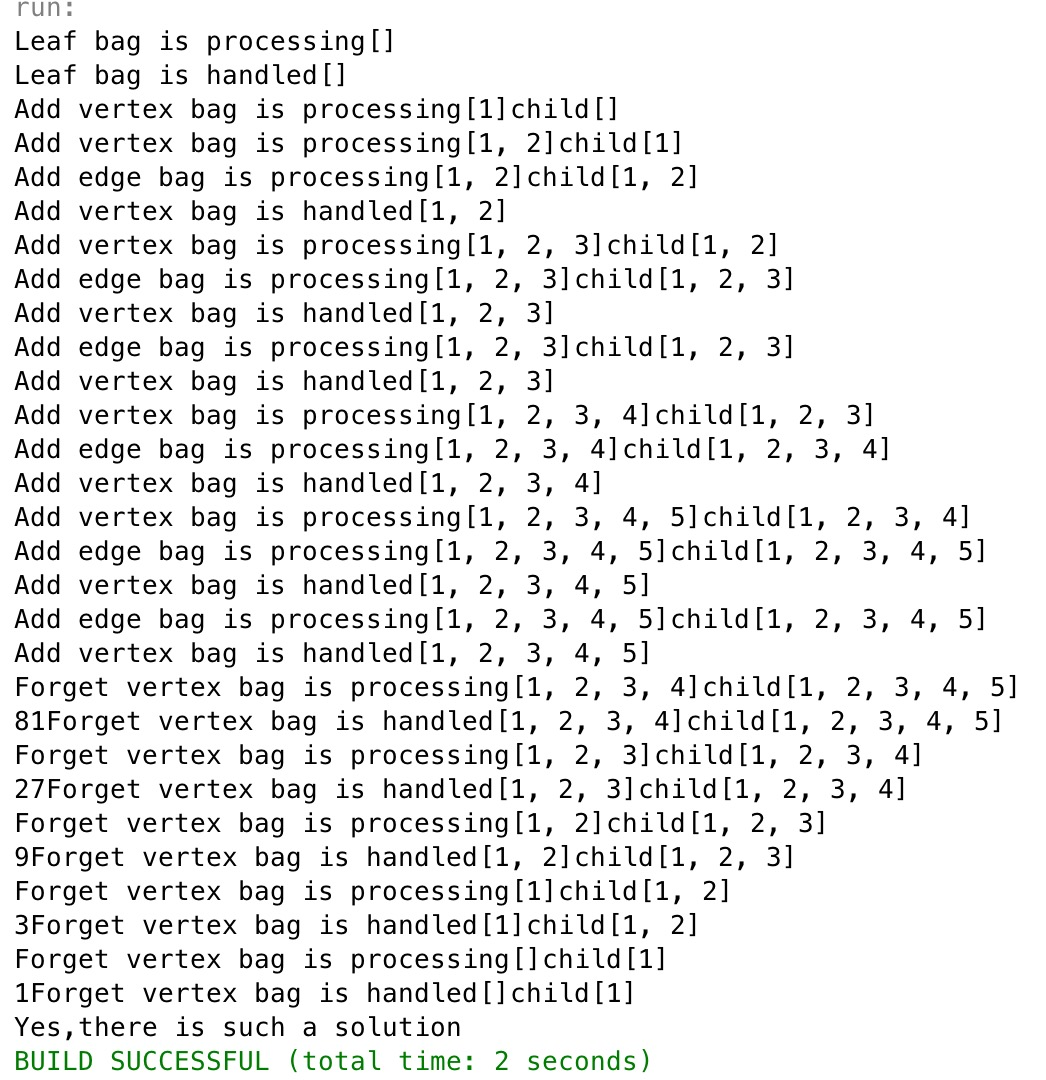
\includegraphics[width=.8\textwidth]{a11.png}
  \caption{Result of 5 vertices graph}
\end{figure}
Results for 7 vertices graph:
\begin{figure}[H] 
  \centering
  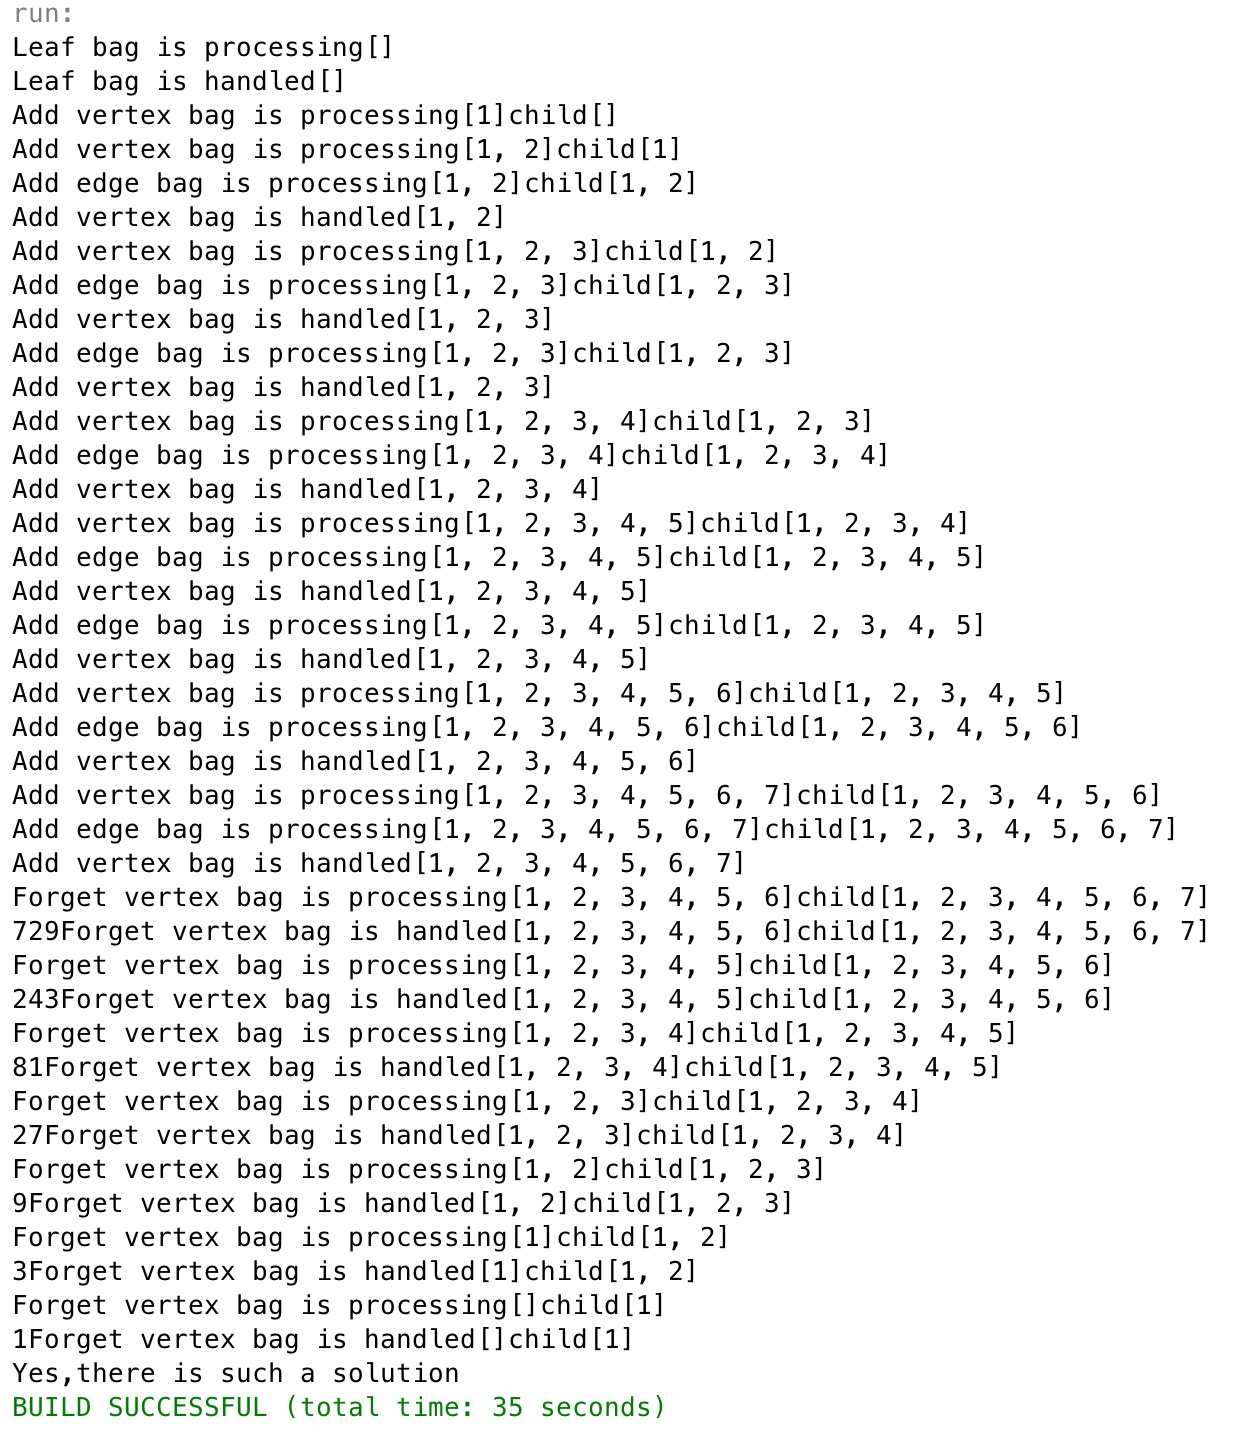
\includegraphics[width=.8\textwidth]{a12.png}
  \caption{Result of 5 vertices graph}
\end{figure}


\FloatBarrier
\section{Task division}
\subsection{Stefan Majoor}
\begin{itemize}
 \item Abstract, Sections~\ref{sec:splitsolve} (SplitSolve), \ref{sec:rand} (Randomized Algorithm) and \ref{sec:comparison} (Comparison) of the report.
 \item Implementation of the randomized algorithm
 \item Implementation of the randomized density algorithm
 \item Implementation of the reductions rules used in iterative compression
 \item Implementation of the split solver
 \item First implementation of Simple Disjoint Algorithm
 \item Optimization of kernelization
\end{itemize}

\subsection{Huib Donkers}
\begin{itemize}
 \item Section~\ref{sec:itcomp} (Iterative compression)
 %and Appendix~\ref{app:itcomp} (Experimental results Iterative Compression)
 of the report.
 \item Implementation of and improvements to the iterative compression algorithm
\end{itemize}

\subsection{Henk Alkema}
\begin{itemize}
 \item Subsection~\ref{sec:treewidth1} (Making tree decompositions) and subsection~\ref{sec:treewidth3} (Comparing found treewidths and FVS sizes) of the report.
 \item Implementation of and improvements to the tree decomposition creating algorithm.
 \item Subsection
\end{itemize}

\subsection{Xi Junquan}
\begin{itemize}
 \item Subsection~\ref{sec:dynamic program} (Dynamic programming based on given nice path decomposition) of the report.
 \item Implementation of and improvements to the dynamic programming for deciding whehter solution exists.
\end{itemize}

\subsection{Leo van Gansewinkel}
\begin{itemize}
 \item 
\end{itemize}

\subsection{Christopher Ankomah}
\begin{itemize}
 \item 
\end{itemize}



\end{document}
